\documentclass{article}
\usepackage[
        a4paper,
        left=3cm,
        right=3cm,
        top=3cm,
        bottom=4cm,
]{geometry}
\usepackage{graphicx}
\usepackage{caption}
\usepackage{enumerate}
\usepackage{subcaption}
\usepackage[procnames]{listings}
\usepackage{color}
\usepackage{amsmath}
\usepackage{hyperref}

\title{Lab Assignement 0}
\date{\today}
\author{
	Karamoulas Eleftherios - S3261859\\
	Tzafos Panagiotis - S3302148\\
}

\begin{document}
\maketitle
\section{Answers for Lab 0}
\begin{enumerate}
\item
After our experiments keeping 2 constants and sweeping 1 of the factors we came to the conclusion that when we sweep Rin low values give as spare spikes and when the value gets increased spikes occur more often until Rin reaches a high value that zeros the v(n) and in this case we have very few spikes. When we sweep tau because he is the divisor in our equation low values of tau give frequent spikes and the increase of tau has as a result to reach a point where we have none spikes. Last the sweep of theta as its the factor that limits our v(n) when its gonna become zero again when we have small theta the spikes are often and while theta rices the frequency of spikes drops down.
\item
Something more i guess.
\begin{figure}[!h]
    \centering
    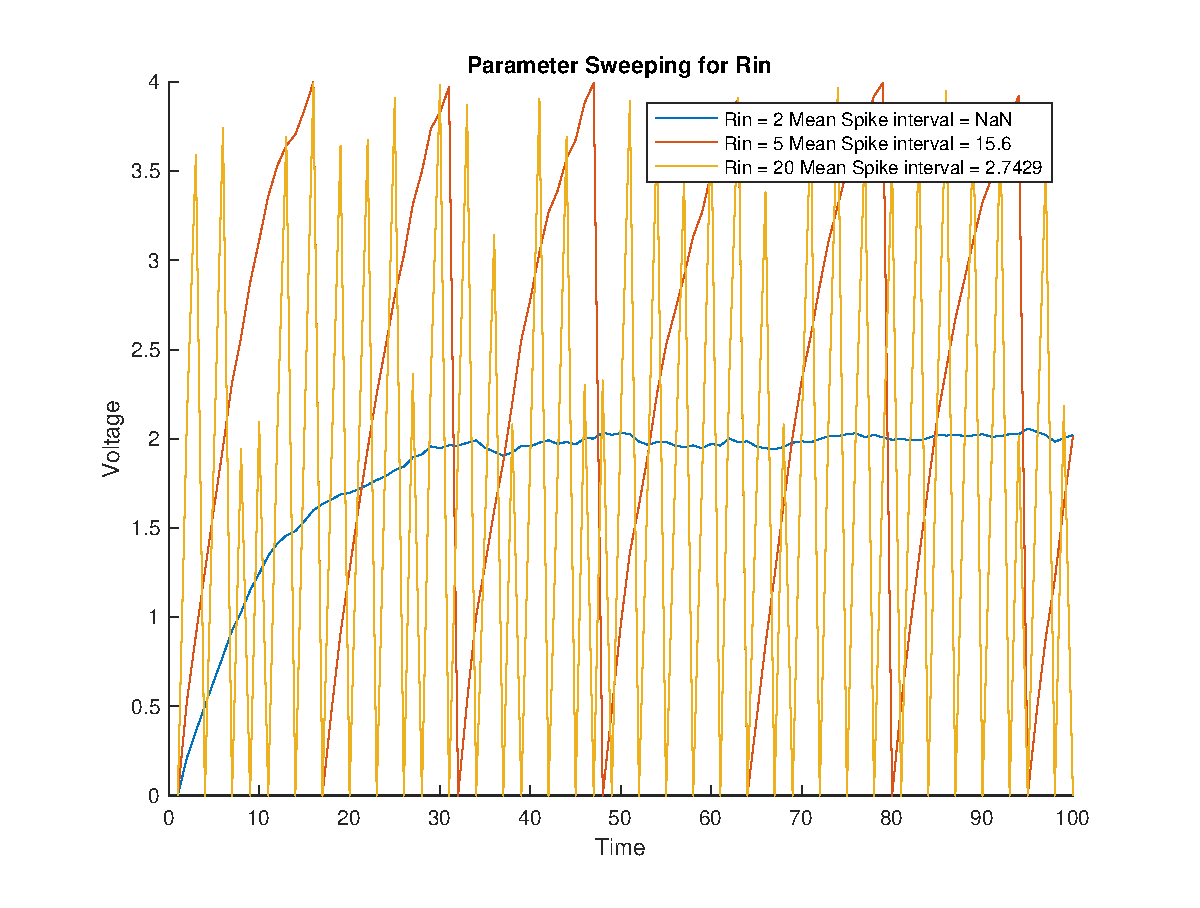
\includegraphics[width=0.7\textwidth]{im/Rin-Sweep.eps}
    \caption{R-sweep}
    \label{fig:plot}
  \end{figure}
  \begin{figure}[!h]
    \centering
    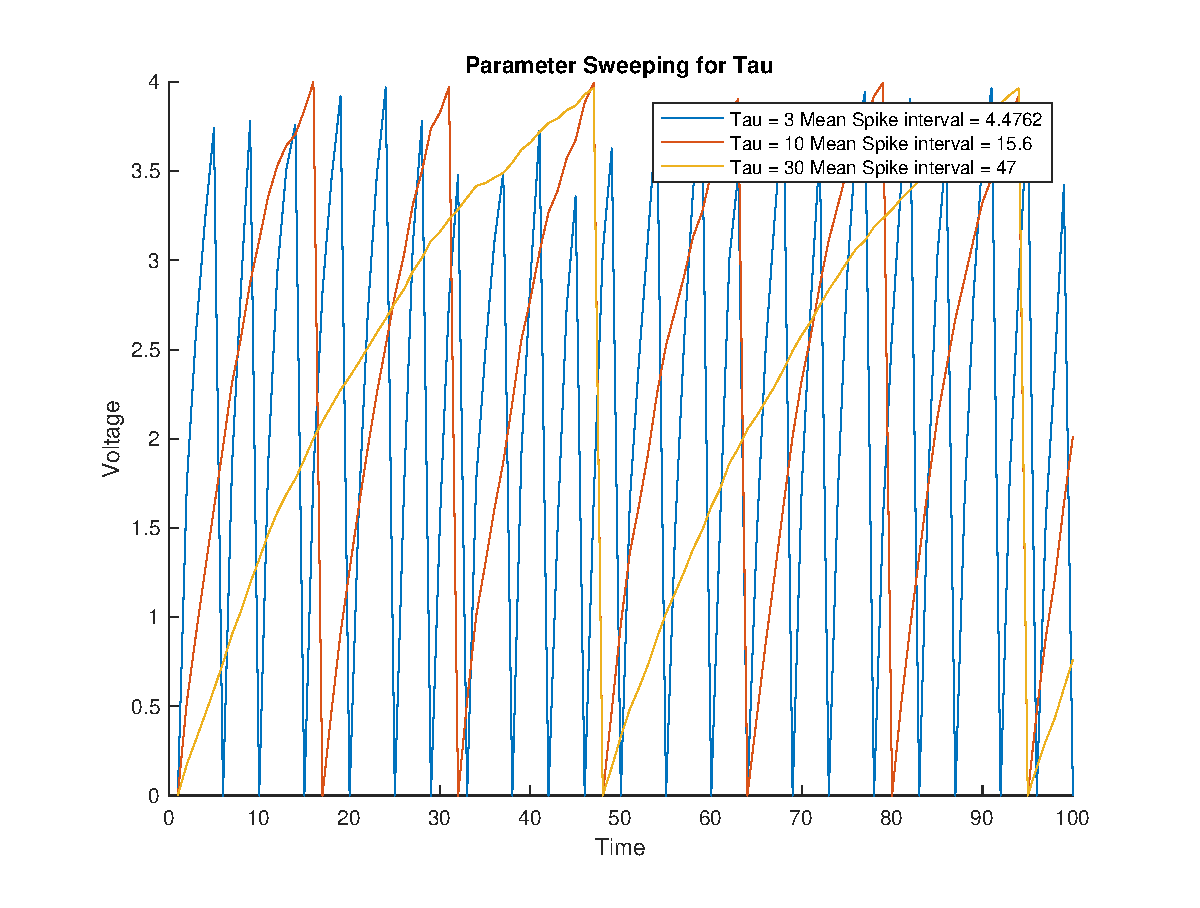
\includegraphics[width=0.7\textwidth]{im/Tau-Sweep.eps}
    \caption{Tau-sweep}
    \label{fig:plot}
  \end{figure}
  \begin{figure}[!h]
    \centering
    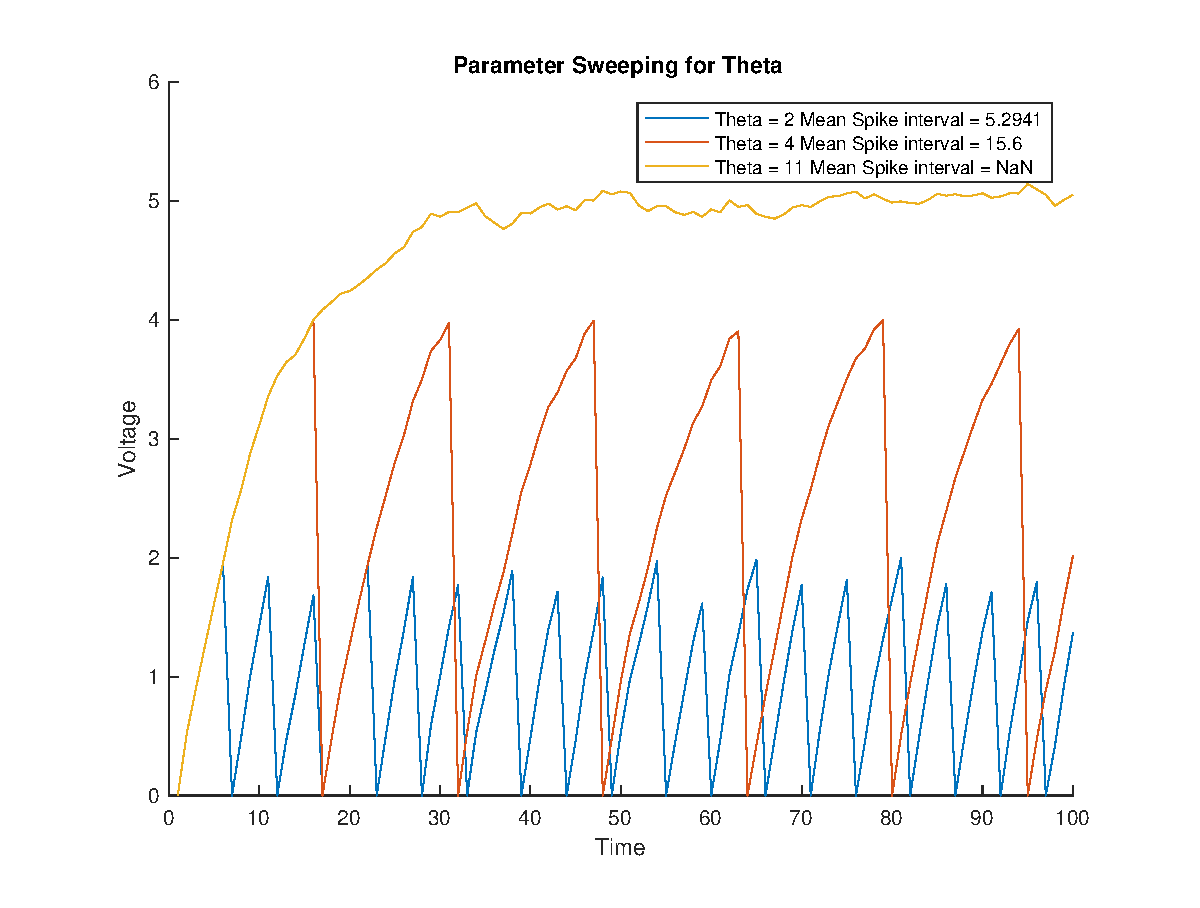
\includegraphics[width=0.7\textwidth]{im/Theta-Sweep.eps}
    \caption{Theta-sweep}
    \label{fig:plot}
  \end{figure}
\item
\lstinputlisting[caption={integrator.m},label={code:bar}]{src/noisyifneuron.m}
\lstinputlisting[caption={isi.m},label={code:bar}]{src/isi.m}
\end{enumerate}
\end{document}